% !TEX root = ../main.tex
% chktex-file 46
\chapter{Related Work}%
\label{sec:related}

Before combining \ac{lta} and \ac{gcr} as described in \cref{sec:intro:goals}, we first give an overview of the state-of-the-art in both fields of research.
First the existing \ac{lta} methods for unstructured set inputs are described.
Then we will look at the two main families of \ac{gcr} methods:
\begin{enumerate*}
	\item Vector representation methods
	\item Graph neural networks
\end{enumerate*}.

\section{Learning to Aggregate}%
\label{sec:related:lta}

The class of \ac{lta} problems was first described by \citet{Melnikov2016}.
There an input instance is understood as a composition $\bm{c}$ of so-called constituents $c_i \in \bm{c}$, i.e.\ as a variable-size multiset with $n = |\bm{c}|$.
The assumption in \ac{lta} problems is that for all constituents $c_i$ a local score $y_i \in \mathcal{Y}$ is either given or computable.
The set of those local scores should be indicative of the overall score $y \in \mathcal{Y}$ of the composition $\bm{c}$.
\ac{lta} problems typically require two subproblems to be solved:
\begin{enumerate}[label=\textbf{\arabic*.}]
	\item \textbf{Aggregation:}
		A variadic aggregation function $\mathcal{A}: \mathcal{Y}^{*} \to \mathcal{Y}$ that estimates composite scores has to be learned, i.e.\@ $y_i \approx \hat{y} = \mathcal{A}(y_{1}, \dots, y_{n})$.
		Typically the aggregation function $\mathcal{A}$ should be associative and commutative to fit with the multiset-structure of compositions.
	\item \textbf{Disaggregation:}
		In case the constituent scores $y_i$ are not given, they have to be derived from a constituent representation, e.g.\ a vector $x_i \in \mathcal{X}$.
		To learn this derivation function $f: \mathcal{X} \to \mathcal{Y}$, only the constituent vectors ${\{x_i\}}_{i = 1}^{n}$ and the composite score $y$ is given.
		Thus the constituent scores $y_i$ need to be \textit{disaggregated} from $y$ in order to learn $f$.
\end{enumerate}
\begin{figure}
	\centering
	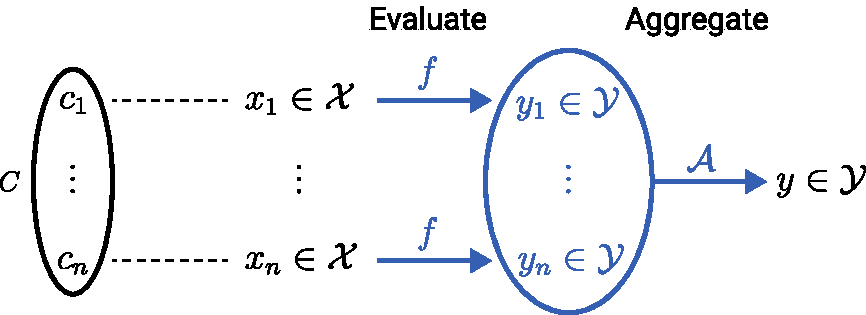
\includegraphics[width=0.7\linewidth]{gfx/related-work/lta-overview.pdf}
	\caption{Overview of the structure of LTA for multiset compositions.}\label{fig:related:lta-overview}
\end{figure}
Overall \ac{lta} can be understood as the joint problem of learning the aggregation function $\mathcal{A}$ and the local score derivation function $f$.
Two main approaches to represent the aggregation function in \ac{lta} problems have been explored.

\subsection{Uninorm-Aggregation}%
\label{sec:related:lta:uninorm}

The first approach uses \textit{uninorms}~\cite{Melnikov2016} to do so.
There the basic idea is to express composite scores as fuzzy truth assignments $y \in [0, 1]$.
Such a composite assignment $y$ is modeled as the result of a parameterized logical expression of constituent assignments $y_i \in [0, 1]$.
As the logical expression that thus effectively aggregates the constituents, a uninorm $U_{\lambda}$ is used.
Depending on the parameter $\lambda \in [0, 1]$, $U_{\lambda}$ combines a t-norm $T$ and a t-conorm $S$ which are continuous generalizations of logical conjunction and disjunction respectively.
One popular choice of norms are the so-called Łukasiewicz norms:
\begin{align}
	\text{t-norm } T(a, b) &:= \max \{ 0, a + b - 1 \}, \quad\text{t-conorm } S(a, b) := \min \{ a + b, 1 \} \nonumber \\
	\text{uninorm } U_\lambda(a, b) &:= \begin{cases}
		\lambda T\left(\frac{a}{\lambda}, \frac{b}{\lambda}\right) & \text{if } a, b \in [0, \lambda] \\
		\lambda + (1 - \lambda) S\left(\frac{a - \lambda}{1 - \lambda}, \frac{b - \lambda}{1 - \lambda}\right) & \text{if } a, b \in [\lambda, 1] \\
		\lambda \min \{ a, b \} & \text{else}
	\end{cases}
\end{align}
At the extreme points $(0, 0)$, $(0, 1)$, $(1, 0)$ and $(1, 1)$, $T$ and $S$ coincide with the Boolean operators $\land$ and $\lor$;
the values at all other points are interpolated as shown in \cref{fig:related:logic-norms}.
The uninorm $U_\lambda$ uses the conjunctive t-norm $T$ for values below the threshold $\lambda$ and the disjunctive t-conorm $S$ for values above the threshold.
$U_\lambda$ therefore smoothly interpolates between a conjunctive and disjunctive operator with the extreme points $U_1 = T$ and $U_0 = S$.
\begin{figure}[h]
	\centering
	\begin{tikzpicture}
		\begin{axis}[
			title={t-norm $T$ ($\land$)},
			xlabel=$a$,
			ylabel=$b$,
			xlabel style={xshift=0.2cm, yshift=0.15cm},
			ylabel style={xshift=-0.2cm, yshift=0.15cm},
			tick label style={font=\scriptsize},
			width=0.33\textwidth,
			colormap = {bluered}{color(0cm) = (t_blue); color(1cm) = (t_red)}
		]
			\addplot3[
				mesh,
				samples=12,
				domain=0:1,
				domain y=0:1
			]{max(x + y - 1, 0)};
		\end{axis}
	\end{tikzpicture}
	\begin{tikzpicture}
		\begin{axis}[
			title={t-conorm $S$ ($\lor$)},
			xlabel=$a$,
			ylabel=$b$,
			xlabel style={xshift=0.2cm, yshift=0.15cm},
			ylabel style={xshift=-0.2cm, yshift=0.15cm},
			tick label style={font=\scriptsize},
			width=0.33\textwidth,
			colormap = {bluered}{color(0cm) = (t_blue); color(1cm) = (t_red)}
		]
			\addplot3[
				mesh,
				samples=12,
				domain=0:1,
				domain y=0:1
			]{min(x + y, 1)};
		\end{axis}
	\end{tikzpicture}
	\begin{tikzpicture}
		\begin{axis}[
			title={uninorm $U_{0.5}$ ($\land$/$\lor$)},
			xlabel=$a$,
			ylabel=$b$,
			xlabel style={xshift=0.2cm, yshift=0.15cm},
			ylabel style={xshift=-0.2cm, yshift=0.15cm},
			tick label style={font=\scriptsize},
			width=0.33\textwidth,
			colormap = {bluered}{color(0cm) = (t_blue); color(1cm) = (t_red)}
		]
			\addplot3[
				mesh,
				samples=12,
				domain=0:1,
				domain y=0:1
			]{(x <= 0.5 && y <= 0.5) * 0.5 * max(2 * (x + y) - 1, 0) + (x > 0.5 && y > 0.5) * (0.5 + 0.5 * min(2 * (x + y - 1), 1)) + (!(x <= 0.5 && y <= 0.5) && !(x > 0.5 && y > 0.5)) * min(x, y)};
		\end{axis}
	\end{tikzpicture}
	\caption{The Łukasiewicz norms and the corresponding uninorm for $\lambda = 0.5$.}\label{fig:related:logic-norms}
\end{figure}

Since t-norms and t-conorms are commutative and associative they can also be applied to non-empty sets of arbitrary size, i.e. $T(\{ y_1, \dots, y_n \}) = T(y_1, T(\{ y_2, \dots, y_n \}))$ with fixpoint $T(\{ y \}) = y$.
Using this extension, a uninorm $U_\lambda$ can be applied to sets which turns it into a parameterized aggregation function $\mathcal{A}_\lambda: {[0, 1]}^* \to [0, 1]$.
In this simple model the \ac{lta} aggregation problem boils down to the optimization of $\lambda$.
The \ac{lta} disaggregation problem was not considered in the uninorm approach~\cite{Melnikov2016}, i.e.\ the constituent scores ${\{ y_i \}}_{c_i \in \bm{c}}$ are assumed to be given.

\subsection{\acs*{owa}-Aggregation}%
\label{sec:related:lta:owa}

Recently \citet{Melnikov2019} have looked at an alternative class of aggregation functions.
Instead of using fuzzy logic to describe score aggregation, \ac{owa} operators were used.
\ac{owa} aggregators work by sorting the input scores and then weighting them based on their sort position, i.e.\ %
\begin{align*}
	\mathcal{A}_{\lambda}(y_1, \dots, y_n) := \sum_{i = 1}^n \lambda_i y_{\pi(i)},
\end{align*}
where $\lambda \in \mathbb{R}^n$ is a weight vector with ${\|\lambda\|}_1 = 1$ and $\pi$ is a sorting permutation of the input scores with $y_i < y_j \Rightarrow \pi(i) < \pi(j)$. % chktex 21
Depending on the choice of the vector $\lambda$, the \ac{owa} function $\mathcal{A}_\lambda$ can express common aggregation functions like
$\min$ (if $\lambda = (1, 0, \dots, 0)$),
$\max$ (if $\lambda = (0, \dots, 0, 1)$)
or the arithmetic mean (if $\lambda = \left(\frac{1}{n}, \dots, \frac{1}{n}\right)$).

To deal with varying composition sizes $n$, the weights ${\{ \lambda_i \}}_{i = 1}^{n}$ can however not be statically assigned.
Instead they are interpolated using a so-called \ac{bum} function $q: [0, 1] \to [0, 1]$.
It takes constituent positions that are normalized to the unit interval, i.e.\ $\frac{i}{n} \in [0, 1]$.
The \ac{bum} function $q$ is then used to interpolate a weight for any normalized sort position via $\lambda_i := q\left(\frac{i}{n}\right) - q\left(\frac{i - 1}{n}\right)$.
Because $q$ is monotone with $q(0) = 0$ and $q(1) = 1$, it always holds that ${\|\lambda\|}_1 = q(1) - q(0) = 1$. % chktex 21
Using this model, the aggregation problem boils down to optimizing the shape of $q$.

In the described \ac{owa} approach~\citet{Melnikov2019} the \ac{bum} function $q$ is modeled as a piecewise linear spline.

\section{Graph Regression and Classification}%
\label{sec:related:gcr}

\subsection{Graph Embeddings}%
\label{sec:related:gcr:embed}

\subsection{Graph Kernels}%
\label{sec:related:gcr:kernel}

\subsection{Graph Neural Networks}%
\label{sec:related:gcr:nn}

\subsubsection{Spatial GNNs}

\subsubsection{Spectral GNNs}
